%===========================================================================


\section{Equity Analysis \texorpdfstring{[E]}{[E]}}
\label{sec:equity}
%===========================================================================

\subsection{What the Subgroup Strata Are}
\label{sec:equity_strata}

Two properties of MIMIC-IV's administrative record govern how this section is
read.

\paragraph{Strata are documentation categories.}
\texttt{race} in MIMIC-IV is a single code assigned at registration. Its levels
mix broad categories with more granular ones drawn from the same population:
``White'' and ``White -- Other European'' are separate levels, as are ``Asian''
and ``Asian -- Chinese''. A stay carries exactly one code, so the levels
partition the cohort, but they do not partition it into disjoint
\emph{populations}: the reference level ``White'' is a residual category
comprising stays not assigned a more specific European code, and a contrast
against it is a contrast against that residual. ``Unknown'' and ``Unable to
obtain'' record the \emph{absence} of an answer; they are retained because the
completeness of the record is informative (Section~\ref{sec:label_sens_subgroup})
but are not demographic groups.

\paragraph{Event floor.}
The interpretation floor is \pcMinSubgroupEvents{} sepsis onsets, the same as
the external-validation floor (Section~\ref{sec:external_interpretability};
\cite{riley2019sample, collins2024tripodai}). Strata below it are estimated and
tabulated but \textbf{not interpreted}, and are excluded from statements about
spread and from family E1, which therefore contains \pcEquityNContrastsEOne{}
contrasts. Of the racial strata, \pcNSubgroupsAboveFloor{} clear the floor.

\subsection{Performance Disparities by Subgroup \texorpdfstring{[E]}{[E]}}

\begin{table}[H]
    \centering\footnotesize
    \adjustbox{max width=\textwidth}{% GENERATED by thesis_constants.R -- do not edit
\begin{tabular}{lrrcc}
\toprule
\textbf{Racial stratum} & \textbf{Rows} & \textbf{Sepsis} & \textbf{GBT AUROC (95\% CI)} & \textbf{Primary AUROC (95\% CI)} \\
\midrule
White & 317{,}688 & 597 & 0.739 (0.719--0.761) & 0.756 (0.736--0.777) \\
Unknown & 107{,}158 & 235 & 0.773 (0.742--0.803) & 0.773 (0.740--0.804) \\
Black / African American$^\dagger$ & 31{,}716 & 58 & 0.749 (0.676--0.817) & 0.759 (0.685--0.825) \\
Other$^\dagger$ & 22{,}825 & 35 & 0.669 (0.571--0.756) & 0.724 (0.631--0.806) \\
White -- Other European$^\dagger$ & 11{,}768 & 18 & 0.672 (0.566--0.780) & 0.730 (0.600--0.846) \\
Asian$^\dagger$ & 6{,}543 & 16 & 0.765 (0.625--0.886) & 0.841 (0.726--0.929) \\
Hispanic / Latino -- Puerto Rican$^\dagger$ & 6{,}462 & 16 & 0.624 (0.448--0.792) & 0.702 (0.546--0.845) \\
Asian -- Chinese$^\dagger$ & 5{,}386 & 13 & 0.601 (0.398--0.802) & 0.701 (0.511--0.869) \\
\bottomrule
\end{tabular}
}
    \caption{AUROC by racial stratum (Variant B, temporal test) with 95\%
    stay-level cluster-bootstrap intervals, stratified within stratum,
    $B = 2{,}000$, ordered by exposure. $\dagger$ marks strata with fewer than
    \pcMinSubgroupEvents{} sepsis onsets, which are neither interpreted nor
    entered into family E1 (Section~\ref{sec:equity_strata}).
    \textbf{[E] exploratory.}}
    \label{tab:equity_performance}
\end{table}

The spread of subgroup point estimates is not commensurable with the
model-class and label spreads of Section~\ref{sec:decomposition}: those are
whole-cohort contrasts with one factor varied, whereas a subgroup range is the
extreme order statistic of separate estimates on disjoint slices with few
events, and is biased upward by construction even when every underlying value
is identical. The apparent spread largely reflects how few events the small
strata contain. Of the racial strata,
\pcNSubgroupsAboveFloor{} carry at least \pcMinSubgroupEvents{} onsets; the
remaining \pcEquityRaceBelowFloorN{} are estimated on counts between
\pcEquityRaceBelowFloorMin{} and \pcEquityRaceBelowFloorMax, and their
intervals are correspondingly wide.

Table~\ref{tab:equity_contrasts} therefore reports contrasts against the
reference level on the same bootstrap replicates.

\begin{table}[H]
    \centering\footnotesize
    \adjustbox{max width=\textwidth}{% GENERATED by thesis_constants.R -- do not edit
\begin{tabular}{llrlcrr}
\toprule
\textbf{Variable} & \textbf{Stratum} & \textbf{Sepsis} & \textbf{Model} & \textbf{$\Delta$AUROC vs.\ reference (95\% CI)} & \textbf{$p$} & \textbf{$q_{\text{BH}}$} \\
\midrule
Insurance & Private & 251 & Gbt & $+0.050$ ($+0.012$--$+0.088$) & 0.011 & 0.066 \\
Insurance & Private & 251 & Primary & $+0.039$ ($+0.003$--$+0.077$) & 0.033 & 0.099 \\
Race & Unknown & 235 & Gbt & $+0.033$ ($-0.003$--$+0.069$) & 0.067 & 0.134 \\
Race & Unknown & 235 & Primary & $+0.017$ ($-0.022$--$+0.055$) & 0.387 & 0.580 \\
Insurance & Medicaid & 183 & Primary & $+0.008$ ($-0.036$--$+0.052$) & 0.683 & 0.819 \\
Insurance & Medicaid & 183 & Gbt & $-0.003$ ($-0.049$--$+0.046$) & 0.888 & 0.888 \\
\bottomrule
\end{tabular}
}
    \caption{Exploratory family E1 in full: all \pcEquityNContrastsEOne{}
    subgroup AUROC contrasts clearing the \pcMinSubgroupEvents{}-event floor,
    across race, language and insurance and for both fitted models, ordered by
    adjusted $p$-value. $q_{\text{BH}}$ is the Benjamini--Hochberg adjusted
    value over the whole family. \textbf{No contrast is significant}; two
    unadjusted intervals exclude zero. The reference level is the largest
    stratum of its variable (Section~\ref{sec:equity_strata}).
    \textbf{[E] exploratory.}}
    \label{tab:equity_contrasts}
\end{table}

Applying the floor leaves \pcEquityNContrastsEOne{} contrasts in family E1
across all three equity variables and both models, and \textbf{none survives
false-discovery correction}. The smallest adjusted value in the family belongs
to a contrast on insurance rather than on race: \pcEquityTopEOneLevel{}
insurance against the Medicare reference, \pcEquityTopEOneDelta{} AUROC for the
gradient-boosted model, with a bootstrap interval of
[\pcEquityTopEOneCiLo, \pcEquityTopEOneCiHi] and
$q_{\text{BH}} = \pcEquityTopEOneQ$.

Its interval excludes zero but its adjusted $p$-value does not clear the
threshold. The corrected verdict is the one read here, because the protocol
(§9) fixed the scope of the equity analysis but not the levels, reference or
direction of any contrast; the contrast is reported but not claimed.

Of the racial strata, only two carry enough events to be interpreted, and one
of them is \emph{Unknown}, a missingness category
(Section~\ref{sec:equity_strata}). \textbf{The study therefore contains no
adequately powered comparison between two racial strata that both record a
demographic answer.} The study is \textbf{underpowered to detect subgroup
disparities}: even above the event floor, the intervals are compatible both
with a stratum being served materially worse than the reference and with its
being served slightly better.

Wang et al.'s \cite{wang2022equity} finding of degraded performance for Asian,
Hispanic and Spanish-speaking patients concerns mortality prediction
(Section~\ref{sec:equity_lit}), and the corresponding strata here fall below the
event floor, so it is neither confirmed nor contradicted. The point estimates
for these strata lie below the reference under GBT, in the direction Wang et
al.\ report, but are not interpreted.

\begin{figure}[H]
    \centering
    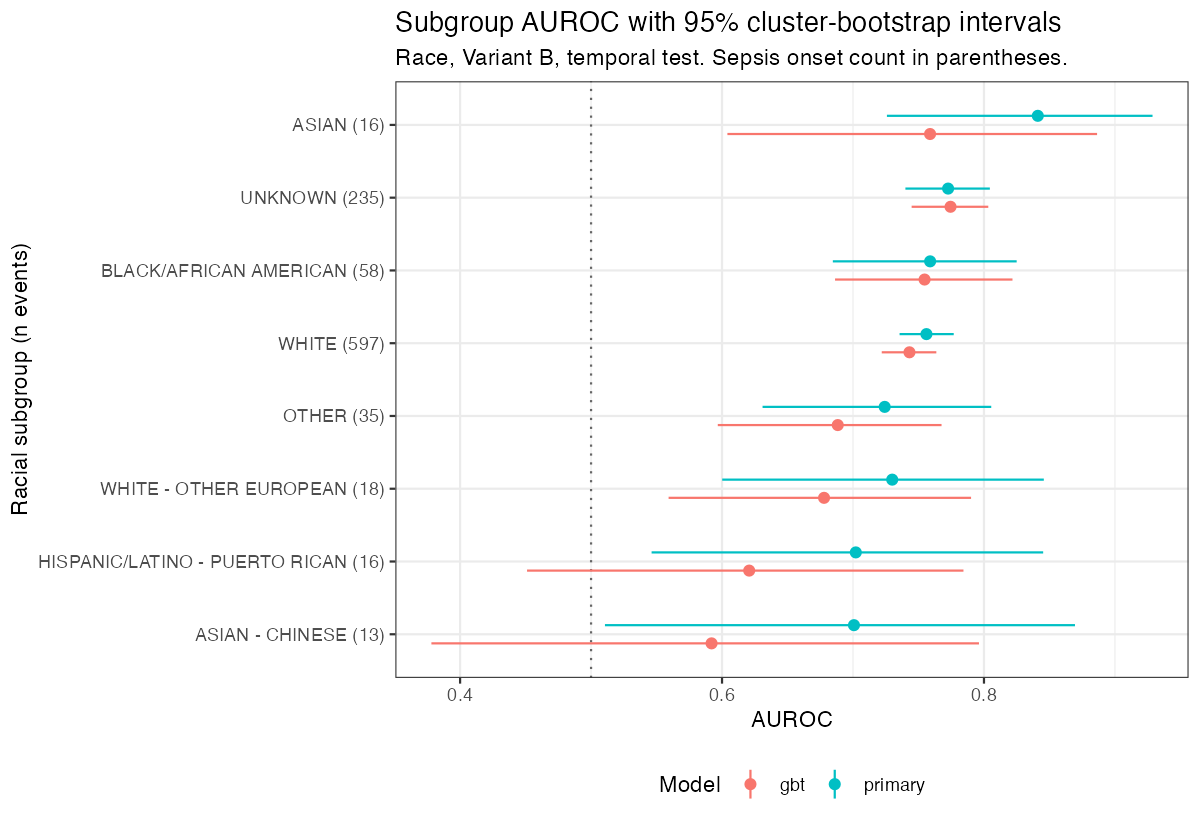
\includegraphics[width=0.92\textwidth]{images/12_subgroup_auroc_ci.png}
    \caption{AUROC by racial subgroup with 95\% stay-level cluster-bootstrap
    intervals (Variant B, temporal test); sepsis onset count in parentheses.
    Interval width is governed almost entirely by the stratum event count, and
    several intervals reach the 0.5 chance line.}
    \label{fig:auroc_by_race}
\end{figure}

\subsection{Label Sensitivity by Subgroup \texorpdfstring{[E]}{[E]}}
\label{sec:label_sens_subgroup}

\begin{table}[H]
    \centering\footnotesize
    \adjustbox{max width=\textwidth}{% GENERATED by thesis_constants.R -- do not edit
\begin{tabular}{lrcccc}
\toprule
\textbf{Racial group} & \textbf{Stays} & \textbf{A (\%)} & \textbf{B (\%)} & \textbf{C (\%)} & \textbf{Range (pp, 95\% CI)} \\
\midrule
White & 40{,}212 & 9.4 & 9.6 & 18.6 & 9.3 (8.9--9.7) \\
Unknown & 7{,}264 & 11.6 & 12.8 & 23.9 & 12.3 (11.3--13.3) \\
Black / African American & 4{,}929 & 9.3 & 9.1 & 19.0 & 9.9 (9.0--11.1) \\
Other & 2{,}254 & 8.8 & 9.8 & 17.5 & 8.7 (7.1--10.2) \\
Unable to obtain & 1{,}629 & 9.7 & 11.1 & 22.5 & 12.8 (10.7--14.9) \\
White -- Other European & 1{,}589 & 9.4 & 7.7 & 16.6 & 8.9 (7.2--10.7) \\
Asian & 799 & 10.5 & 11.5 & 21.3 & 10.8 (8.3--13.8) \\
Asian -- Chinese & 721 & 10.1 & 11.1 & 19.0 & 8.9 (6.4--11.9) \\
\bottomrule
\end{tabular}
}
    \caption{Percentage of stays labelled as septic by racial subgroup and label
    variant, with a 95\% stratified cluster-bootstrap interval on the A--C
    range. The fraction roughly doubles from Variant A to C across all groups.
    Per-variant intervals are in \texttt{12\_subgroup\_labelsens\_ci.csv}.
    \textbf{[E] exploratory.}}
    \label{tab:equity_label}
\end{table}

The fraction of patients labelled as septic changes by
\pcLabelSensRangeLo--\pcLabelSensRangeHi{} percentage points across label
variants within each racial stratum. Unlike discrimination, this contrast
survives correction, because it is a stay-level proportion computed on the full
\pcNStays{}-stay cohort rather than on the few hundred test-window onsets. No
event floor is therefore applied; the construct limitation of
Section~\ref{sec:equity_strata} still applies.

\begin{table}[H]
    \centering\footnotesize
    \adjustbox{max width=\textwidth}{% GENERATED by thesis_constants.R -- do not edit
\begin{tabular}{lrcrr}
\toprule
\textbf{Racial group} & \textbf{Stays} & \textbf{$\Delta$ range vs.\ White (pp, 95\% CI)} & \textbf{$p$} & \textbf{$q_{\text{BH}}$} \\
\midrule
Unknown & 7{,}264 & $+3.01$ ($+1.93$--$+4.06$) & 0.001 & \textbf{0.006} \\
Unable to obtain & 1{,}629 & $+3.49$ ($+1.38$--$+5.55$) & 0.002 & \textbf{0.009} \\
Black / African American & 4{,}929 & $+0.62$ ($-0.35$--$+1.87$) & 0.186 & 0.347 \\
Asian & 799 & $+1.48$ ($-1.04$--$+4.50$) & 0.249 & 0.407 \\
Other & 2{,}254 & $-0.63$ ($-2.26$--$+0.98$) & 0.425 & 0.510 \\
White -- Other European & 1{,}589 & $-0.41$ ($-2.10$--$+1.41$) & 0.635 & 0.714 \\
Asian -- Chinese & 721 & $-0.40$ ($-3.02$--$+2.61$) & 0.675 & 0.714 \\
\bottomrule
\end{tabular}
}
    \caption{Difference in label sensitivity (A--C range) against the reference
    group (White). $q_{\text{BH}}$ is adjusted over exploratory family E2, all
    18 label-sensitivity contrasts across race, language and insurance. Two
    racial contrasts survive at $q < 0.05$; across the full family,
    \pcLabelSensNSig{} do (adding Spanish-speaking patients,
    $+\pcLabelSensSpanishPp$ pp, $q = \pcLabelSensSpanishQ$, and privately
    insured patients, $\pcLabelSensPrivatePp$ pp,
    $q = \pcLabelSensPrivateQ$). \textbf{[E] exploratory.}}
    \label{tab:equity_label_contrasts}
\end{table}

\pcLabelSensNSigRace{} racial strata are significantly more label-sensitive
than the reference after false-discovery correction, and \emph{both of them are
missingness categories}: Unknown ($+\pcLabelSensUnknownPp$ pp,
$q = \pcLabelSensUnknownQ$) and Unable to obtain ($+\pcLabelSensUnablePp$ pp,
$q = \pcLabelSensUnableQ$). No stratum recording an actual demographic answer
differs from the reference. Across the full family, Spanish-speaking patients
are more label-sensitive than English-speaking patients
($+\pcLabelSensSpanishPp$ pp, $q = \pcLabelSensSpanishQ$), and privately
insured patients are \emph{less} label-sensitive than Medicare patients
($\pcLabelSensPrivatePp$ pp, $q = \pcLabelSensPrivateQ$).

The significant contrasts involve documentation-related categories and
strata of language and insurance, and may reflect differences in record
completeness; this mechanism was not tested
(Limitation~\ref{lim:subgroup}). Of the two equity analyses, only this one is
precise enough to support a claim, and reporting either without the other
would invert which conclusion the data support.

\begin{figure}[H]
    \centering
    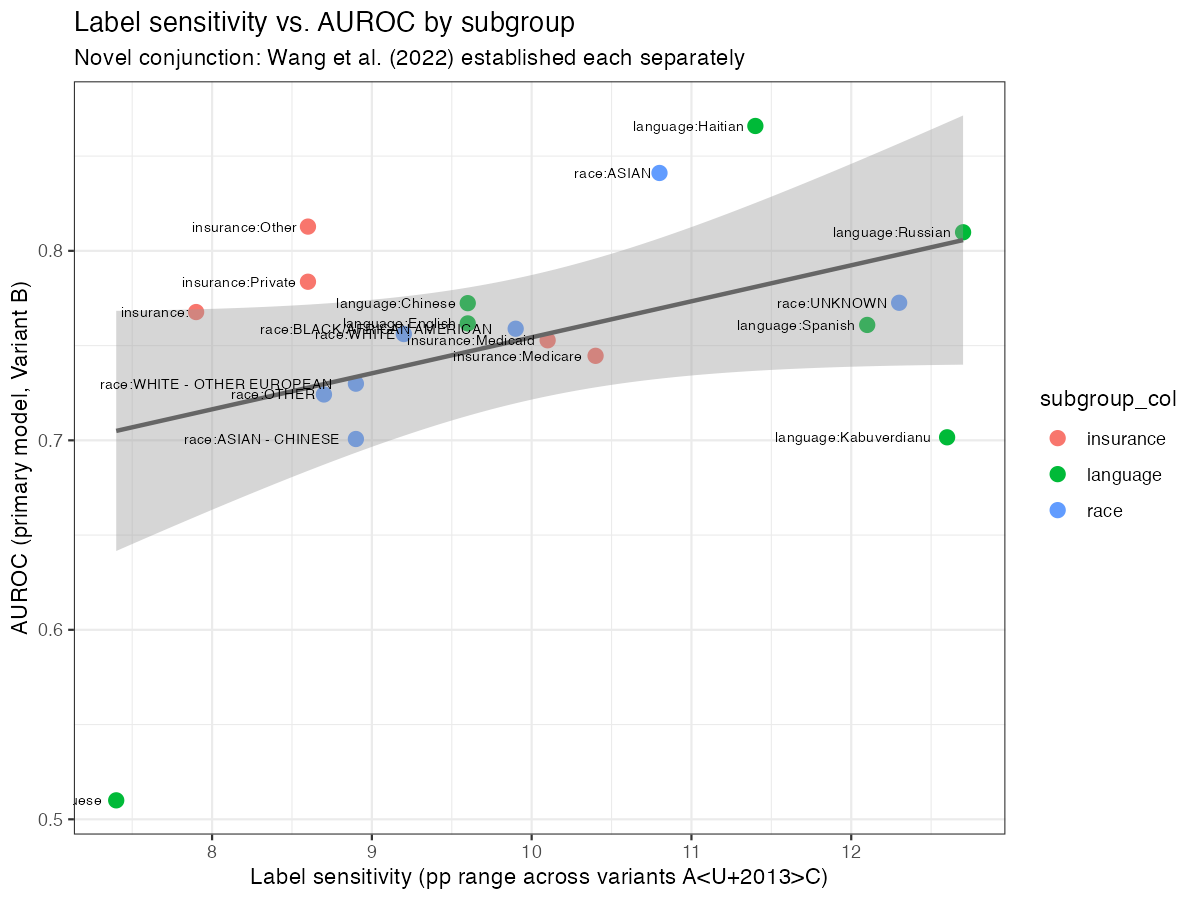
\includegraphics[width=0.85\textwidth]{images/10_label_sens_vs_auroc.png}
    \caption{Label sensitivity (fraction labelled septic) vs.\ AUROC by racial
    subgroup, across all three label variants. No association is tested, and
    the AUROC uncertainty of Figure~\ref{fig:auroc_by_race} is not shown.
    \textbf{[E] exploratory, visual only.}}
    \label{fig:label_sens_vs_auroc}
\end{figure}
